\PassOptionsToPackage{dvipsnames,table}{xcolor}
\documentclass[10pt]{beamer}
\usepackage{Cours}

\begin{document}

\input{\detokenize{/home/fenarius/Travail/Cours/cpge-info/latex//MacrosCours.tex}}

% Numéro et titre de chapitre
\setcounter{numchap}{0}
\newcommand{\Ctitle}{\cnum Notions d'architecture et de système}

\makess{Architecture des ordinateurs}
\begin{frame}{\Ctitle}{\stitle}
	\begin{block}{Modèle de Von Neumann}
		\begin{itemize}
			\item<1-> Les ordinateurs modernes sont construits autour d'un modèle défini par le mathématicien John Von Neumann dans les années 1940 appelé \textcolor{blue}{Architecture de Von Neumann}
			\item<2-> Dans ce modèle, l'ordinateur se décompose :
				\begin{itemize}
					\item<3-> La \textcolor{blue}{mémoire} qui stocke les données et les programmes (sous forme de 0 et de 1).
					\item<4-> L'\textcolor{blue}{unité arithmétique et logique {\sc ual}} qui effectue les opérations arithmétiques (addition, soustraction, \dots) et logiques (conjonctions, négations, \dots) sur les données.
					\item<5-> L'\textcolor{blue}{unité de contrôle} chargé de l'ordre des opérations et de la récupération des données en mémoire.
					\item<6-> Les dispositifs d'\textcolor{blue}{entrée} (ex : clavier, souris, réseau, \dots), et de \textcolor{blue}{sortie} (ex : écran, imprimante, \dots) des données
				\end{itemize}
		\end{itemize}
	\end{block}
\end{frame}


\begin{frame}{\Ctitle}{\stitle}
	
	\begin{block}{Schéma représentant l'architecture de Von Neumann :}
		\rnode{cmp}{\psframe[linewidth=0.8pt,linecolor=Sepia](3.2,0)(8.8,-5)}
		\rput(6,-1.4){\rnode{cpu}{\psshadowbox[shadowsize=1pt,framesep=0.5cm]{\makebox[4cm]{\raisebox{1cm}{\textcolor{BrickRed}{\textbf{\faMicrochip \ CPU}} } } }}}
		\onslide<2->{\rput(4.5,-1.8){\rnode{ual}{\psframebox[framearc=.3,framesep=0.2cm,linewidth=0.4pt]{\makebox[1.2cm]{UAL}}}}}
		\onslide<2->{\rput(7.5,-1.8){\rnode{uc}{\psframebox[framearc=.3,framesep=0.2cm,linewidth=0.4pt]{\makebox[1.2cm]{UC}}}}}
		\onslide<3->{\rput(5.75,-4.2){\rnode{ram}{\psshadowbox[shadowsize=1pt,framesep=0.5cm]{\makebox[4cm]{\textcolor{BrickRed}{\textbf{\faMemory \ Mémoire}}} }}}}
		\onslide<4->{\rput(0.8,-2.4){\rnode{in}{\psshadowbox[shadowsize=1pt,framesep=0.4cm]{\makebox[1.2cm]{\textcolor{blue}{\textbf{Entrées \ \faArrowAltCircleRight}}} }}}}
		\onslide<5->{\rput(10.4,-2.4){\rnode{out}{\psshadowbox[shadowsize=1pt,framesep=0.4cm]{\makebox[1.2cm]{\textcolor{blue}{\textbf{\faArrowAltCircleRight \ Sorties}}} }}}}
		\onslide<6->{\ncline[linecolor=blue, linewidth=2px, offset = 1.5cm]{<->}{ram}{cpu}
			\ncline[linecolor=blue, linewidth=2px, offset = -1.5cm]{<->}{ram}{cpu}}
		\onslide<7->{\ncline[linecolor=blue, linewidth=2px,offsetA=-0.2cm,offsetB=-0.37cm,nodesepB=0.4cm]{->}{in}{cpu}
			\ncline[linecolor=blue, linewidth=2px,offsetB=-0.17cm,offsetA=-0.35cm,nodesepA=0.3cm]{->}{cpu}{out}}
		\vspace{5cm}
	\end{block}
\end{frame}

\makess{Système d'exploitation}
\begin{frame}{\Ctitle}{\stitle}	
	\begin{alertblock}{Définition}
		Un \textcolor{red}{système d'exploitation}  (en abrégé \textcolor{red}{OS}, de l'anglais \textit{Operating System}) est un programme (ou ensemble de programme) permettant de
		\onslide<2->{gérer les ressources de l'ordinateur (mémoire, fichier, périphériques, \dots) sur lequel il s'execute}. \\
	\end{alertblock}
	\onslide<3->{\begin{exampleblock}{Exemples}
			Les systèmes d'exploitation les plus répandus à l'heure actuelle sont :
			\begin{itemize}
				\item[\faWindows] <4-> Windows (différentes versions)
				\item[\faLinux] <5-> {\sc gnu}/Linux  (plusieurs centaines de distribution différentes, parmi les plus connus : ubuntu, fedora, archlinux)
				\item[\faAndroid] <6-> Android (smartphone)
				\item[\faApple] <7-> MacOs (ordinateur) et iOS (smartphone)
			\end{itemize}
		\end{exampleblock}}
\end{frame}

%Schéma représentatif
\begin{frame}{\Ctitle}{\stitle}
	\begin{block}{La place du système d'exploitation}
		\setlength{\shadowsize}{1pt}
		\begin{tabularx}{0.9\textwidth}{Y}
			\onslide<2->{\rnode{ut}{\psshadowbox{\makebox[5cm]{\par\noindent\rule[-0.2cm]{0pt}{0.6cm} \textcolor{BrickRed}{\textbf{\faUser \ L'utilisateur}} }} } }           \\
			\\
			\onslide<3->{\rnode{ap}{\psshadowbox{\makebox[5cm]{\par\noindent\rule[-0.2cm]{0pt}{0.6cm} {\textcolor{BrickRed}{\textbf{\faThList \ Les applications}} } }}}}     \\
			\\
			\onslide<6->{\rnode{os}{\psshadowbox{\makebox[5cm]{\par\noindent\rule[-0.2cm]{0pt}{0.6cm} {\textcolor{BrickRed}{\textbf{\faLinux \ Système d'exploitation}}} }}}} \\
			\\
			\onslide<6->{\rnode{or}{\psshadowbox{\makebox[5cm]{\par\noindent\rule[-0.2cm]{0pt}{0.6cm} {\textcolor{BrickRed}{\textbf{\faLaptop \ L'ordinateur}}} }}}}
		\end{tabularx}
		\onslide<4->{\ncline[doubleline=true,offset=1cm,doublesep=3pt,doublecolor=blue,linecolor=blue,linewidth=0.5pt,arrowsize=10pt,arrowinset=0.2,arrowlength=1.2]{->}{ut}{ap}}
		\onslide<4->{\ncline[doubleline=true,offset=1.5cm,doublesep=3pt,doublecolor=blue,linecolor=blue,linewidth=0.5pt,arrowsize=10pt,arrowinset=0.2,arrowlength=1.2]{<-}{ut}{ap}}
		\onslide<5->{\naput{ \textit{\small interagit avec} }}
		\onslide<7->{\ncline[doubleline=true,offset=0cm,doublesep=3pt,doublecolor=blue,linecolor=blue,linewidth=0.5pt,arrowsize=10pt,arrowinset=0.2,arrowlength=1.2]{<-}{ap}{os}}
		\onslide<7->{\ncline[doubleline=true,offset=0.5cm,doublesep=3pt,doublecolor=blue,linecolor=blue,linewidth=0.5pt,arrowsize=10pt,arrowinset=0.2,arrowlength=1.2]{->}{ap}{os}}
		\onslide<7->{\naput{\textit{\small demandent des ressources au}}}
		\onslide<8->{\ncline[doubleline=true,offset=-1cm,doublesep=3pt,doublecolor=blue,linecolor=blue,linewidth=0.5pt,arrowsize=10pt,arrowinset=0.2,arrowlength=1.2]{<-}{os}{or}}
		\onslide<8->{\ncline[doubleline=true,offset=-0.5cm,doublesep=3pt,doublecolor=blue,linecolor=blue,linewidth=0.5pt,arrowsize=10pt,arrowinset=0.2,arrowlength=1.2]{->}{os}{or}}
		\onslide<8->{\naput{\textit{\small gèrent les ressources de		}}}
	\end{block}
\end{frame}

\begin{frame}{\Ctitle}{\stitle}
	\begin{block}{Fonctionnalités d'un système d'exploitation}
		\begin{itemize}
			\item<1-> Gestion des périphériques.
			\item<2-> Donner l'illusion que l'ordinateur est multitâches.
			\item<3-> Gérer les différentes applications utilisées.
			\item<4-> Identifier les utilisateurs.
			\item<5-> Contrôler et distribuer les accès aux ressources de l'ordinateur.
			\item<6-> Gérer le système de fichier.
		\end{itemize}
	\end{block}
\end{frame}

\begin{frame}{\Ctitle}{\stitle}	
	\begin{block}{Le système de gestion de fichiers}
		\begin{itemize}
			\item<1-> L'ensemble des fichiers forme une arborescence démarrant au répertoire \textcolor{Sepia}{\tt /} appelé \textcolor{blue}{racine} (\textit{root}) \hspace{-2cm}.
				\onslide<2->{\pstree[levelsep=0.8cm]{\noeud{blue}{/}}{
						\pstree[levelsep=0.8cm]{\noeud{blue}{bin}}{\Tr{\textcolor{Sepia}{\tt ls}} \Tr{\textcolor{Sepia}{\tt cat}}}
						\noeud{blue}{etc}
						\noeud{blue}{tmp}
						\pstree[levelsep=1cm]{\noeud{blue}{home}}{\noeud{blue}{\footnotesize Pierre} \noeud{blue}{\footnotesize Paul} \noeud{blue}{\footnotesize Jacques}}}}
			\item<3-> Les fichiers où les répertoires sont spécifiés :
				\begin{itemize}
					\item<4-> s'ils commencent par \textcolor{blue}{\tt /} en chemin \textcolor{blue}{absolu} c'est à dire depuis la racine.
					\item<5-> sinon en chemin \textcolor{blue}{relatif} c'est à dire depuis le répertoire courant (le répertoire parent se note alors \textcolor{blue}{\tt ..}).
				\end{itemize}
			\item<6-> Trois type de droits sont définis sur les fichiers et dossiers :
				\begin{itemize}
					\item<6->[{\tt r}] droit de lecture du fichier
					\item<7->[{\tt w}] droit d'écriture  dans le fichier
					\item<8->[{\tt x}] droit d'execution du fichier
				\end{itemize}
		\end{itemize}
	\end{block}
\end{frame}

\makess{Le \textit{shell}}
\begin{frame}{\Ctitle}{\stitle}
	\begin{block}{Interface système : \textit{shell}}
		\begin{itemize}
			\item<1-> Avant l'avènement des interfaces graphiques (et de la souris), l'utilisateur communiquait avec le système d’exploitation via un programme appelé \textcolor{blue}{\textit{shell}} par l'intermédiaire d'un simple clavier et d'une interface en ligne de commande ({\sc cli} en anglais pour \textit{Command Line Interface}).
			\item<2-> Aujourd'hui encore et pour diverses raisons (rapidité, contrôle plus fin de l'ordinateur, récupération d'erreurs, \dots) la ligne de commande reste très utilisée.
			\item<3-> Voici un exemple d'invite de commande :\\
				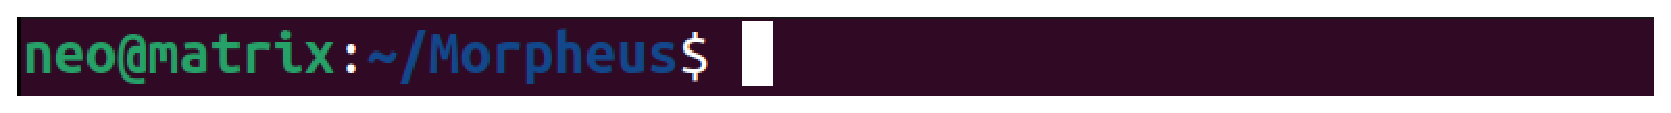
\includegraphics[width=200px]{neo.eps} \\
				On y trouve :
				\begin{itemize}
					\item<4-> Le nom de l'utilisateur ici \textcolor{green}{\tt neo} suivi de \textcolor{green}{\tt @}
					\item<5-> Le nom de l'ordinateur ici \textcolor{green}{\tt matrix} suivi de {\tt :}
					\item<6-> Le chemin du dossier de travail ici \textcolor{blue}{\tt \~{}/Morpheus}  suivi de {\tt :} et du curseur
				\end{itemize}
		\end{itemize}
	\end{block}
\end{frame}

\begin{frame}{\Ctitle}{\stitle}
	\begin{block}{Généralités sur le {\tt shell}}
		\begin{itemize}
			\item<1-> Les commandes ont généralement le format suivant : \\
				\textcolor{blue}{\tt <nom commande> <option> <arguments>} \\
				où les options sont précédées d'un tiret  simple \textcolor{Sepia}{\tt -} ou double \textcolor{Sepia}{\tt -{}-}
			\item<2-> certains caractères spéciaux permettent d'agir sur un ensemble d'arguments : \\
				\begin{tabularx}{0.8\linewidth}{|c|X|}
					\hline
					\textcolor{Sepia}{\tt ?}    & correspond à n'importe quel caractère                      \\
					\hline
					\textcolor{Sepia}{\tt *}    & correspond à n'importe quel suite de caractères            \\
					\hline
					\textcolor{gray}{\tt [...]} & \textcolor{gray}{correspond aux caractères entre crochets} \\
					\hline
				\end{tabularx}
			\item<3-> Le résultat d'une commande peut-être dirigé :
				\begin{itemize}
					\item<4-> Vers un fichier avec \textcolor{Sepia}{\tt >} (avec écrasement si le fichier existe)
					\item<5-> Vers un fichier avec \textcolor{Sepia}{\tt >{}>} (avec ajout en fin si le fichier existe)
					\item<6-> Vers une autre commande avec \textcolor{Sepia}{\tt |} (\textit{pipe})
				\end{itemize}
		\end{itemize}
	\end{block}
\end{frame}

\begin{frame}{\Ctitle}{\stitle}
	\begin{block}{Quelques commandes}
		\begin{description}
			\item<1->[\textcolor{blue}{\tt man}] : affiche l'aide sur une commande
			\item<2->[\textcolor{blue}{\tt pwd}] : affiche le répertoire courant
			\item<3->[\textcolor{blue}{\tt mkdir}] : crée un ou plusieurs dossiers
			\item<4->[\textcolor{blue}{\tt rmdir}] : supprime un dossier
			\item<5->[\textcolor{blue}{\tt mv}] : déplace un dossier ou un fichier
			\item<6->[\textcolor{blue}{\tt ls}] : liste le contenu d'un dossier
				{\footnotesize \begin{itemize}
						\item[{\tt -a}] affiche les fichiers cachés (dont le nom commence par un point)
						\item[{\tt -l}] permet de voir les droits sur les fichiers
						\item[{\tt -i}] permet de voir les inodes
					\end{itemize}}
			\item<7->[\textcolor{blue}{\tt cat}] : écrit le contenu d'un fichier dans le terminal
			\item<8->[\textcolor{blue}{\tt touch}] : crée un fichier vide
			\item<9->[\textcolor{blue}{\tt echo}] : écrit dans le terminal
			\item<10->[\textcolor{blue}{\tt cp}] : copie un fichier
		\end{description}
	\end{block}
\end{frame}

\begin{frame}{\Ctitle}{\stitle}
	\begin{exampleblock}{Exemples}
		\tei{ExArbo.eps}{0.4}{1}{
		A partir du répertoire {\tt Cours}, écrire les commandes pour :
		\begin{enumerate}
			\item<1-> Créer le fichier vide {\tt to\_do} \\
				\onslide<2->{\textcolor{OliveGreen}{\tt touch to\_do}}
			\item<3-> Ecrire dans ce fichier : "{\tt réviser le chapitre 0}" \\
				\onslide<4->{\textcolor{OliveGreen}{\tt echo "réviser le chapitre 0" > to\_do}}
			\item<5-> se déplacer vers le dossier {\tt Factures} (chemin relatif)\\
				\onslide<6->{\textcolor{OliveGreen}{{\tt cd ../../Documents/Factures}}}
			\item<7-> y créer les dossiers {\tt Eau}, {\tt Electricité} et {\tt Téléphone}\\
				\onslide<8-> {\textcolor{OliveGreen}{{\tt mkdir Eau Electricité Téléphone}}}
			\item<9-> lister tous le fichiers contenant {\tt edf}\\
				\onslide<10-> {\textcolor{OliveGreen}{{\tt ls *edf*}}}
			\item<11-> Les déplacer dans le dossier {\tt Electricité}\\
				\onslide<12-> {\textcolor{OliveGreen}{{\tt mv *edf* Electricité}}}
		\end{enumerate}
		}
	\end{exampleblock}
\end{frame}

\begin{frame}{\Ctitle}{\stitle}
	\begin{block}{Droits sur un fichier, {\tt chmod}}
		\begin{itemize}
			\item<2-> Les droits sur un fichier (\textcolor{blue}{\tt r} : lecture, \textcolor{blue}{\tt w} : écriture, \textcolor{blue}{\tt x} exécution) sont définis pour le propriétaire : {\textcolor{blue}{\tt u}} (\textit{user}), le groupe : {\textcolor{blue}{\tt g}} (\textit{groupe}) et les autres :{\textcolor{blue}{\tt o}} (\textit{others}).
			\item<3-> La commande \textcolor{blue}{\tt ls -l} permet d'afficher les droits, par exemple : \\
				{\tt rwxr-x---} indique que l'utilisateur a tous les droits, le groupe peut lire et écrire et les autres n'ont aucun droit.
			\item<4-> La commande \textcolor{blue}{\tt chmod} permet de modifier les droits, à l'aide de {\tt +} (ajout), {\tt -} (retrait), {\tt =} (attribution) ou en notation octale ({\tt r=4, w=2, x=1}).
		\end{itemize}
	\end{block}
	\begin{exampleblock}{Exemples}
		\begin{itemize}
			\item<5->{{\tt chmod u+w } :} \onslide<6->{\footnotesize Ajoute  ({\tt +}) le droit d'écriture ({\tt w}) au propriétaire ({\tt g}) }
			\item<7->{{\tt chmod 700 } :} \onslide<8->{\footnotesize Le propriétaire a tous les droits, les autres et le groupe aucun}
			\item<9->{{\tt chmod og-r } :} \onslide<10->{\footnotesize Enlève ({\tt -}) le droit de lecture ({\tt r}) au groupe et aux autres ({\tt og}) }
			\item<11->{{\tt chmod 544} :} \onslide<12->{\footnotesize Le propriétaire peut lire et exécuter, le groupe et les autres peuvent lire}
		\end{itemize}
	\end{exampleblock}
\end{frame}

\makess{Liens et inodes}
\begin{frame}{\Ctitle}{\stitle}
	\begin{block}{Liens physiques ou symboliques}
		\begin{itemize}
			\item<1-> Les fichiers sont stockés sur le support physique par blocs et retrouvés grâce à leur \textcolor{blue}{inode} (\textit{index node} ou noeud d'index).
			\item<2-> Deux noms de fichiers différents peuvent référencer les mêmes données, ils partagent alors le même inode, on dit que c'est un lien physique (\textit{hardlink}).
			\item<3-> Un lien symbolique (\textit{softlink}) est un fichier indiquant un chemin vers un autre fichier (équivalent d'un raccourci de \textit{Windows}).
			\item<4-> La commande \textcolor{blue}{\tt ln} (resp. \textcolor{blue}{\tt ln -s}) permet de créer un lien physique (resp. symbolique).
		\end{itemize}
	\end{block}
	\begin{exampleblock}{Exemples}
		\begin{itemize}
			\item<5-> {\tt ln important.txt ../Sauvegarde/important.sav} \\
				\onslide<6->{Les deux noms de fichiers font référence aux mêmes données}
			\item<7-> {\tt ln -s important.txt ../Sauvegarde/important.sav} \\
				\onslide<8->{Création d'une simple redirection}
		\end{itemize}
	\end{exampleblock}
\end{frame}

\end{document}
